\chapter{System characterization and results}

In this chapter, efforts to characterize the performance and capabilities of the FO-DOCM system will be detailed. Results obtained with the FO-DOCM device on actual cochlear tissues will be shown. The shortcomings and successes of the apparatus will be detailed, and conclusions will be drawn.

\section{Resolution performance}

\subsection{Measurement of axial resolution}

In Section \ref{sec:axial_res}, predictions were made about the axial resolution achievable by the FO-DOCM system. Here, these predictions are validated and limitations are explained.

% \subsection{Results without AOMs}

% To prevent possibly confounding factors, the system was first tested with the AOMs in place. In this case, the $z$-axis stage was moved in increments of 100 nanometers and the DC voltage from the photodetector was acquired and stored for reach position. This ensures that the distance measured by the $z$-stage is accurate, but requires a smaller overall system gain so as not to saturate the photo-detector. The ``sample'' has been replaced by a mirror for maximum possible SNR.

% \begin{figure}[h!]
% \centering
% 
\includegraphics[width=0.75\textwidth]{Images/missing.png}
% \caption[The point spread function without acousto optic modulators.]{The point spread function without acousto optic modulators. The measured PSF is shown in black, the best fit Gaussian in green, and the predicted PSF in blue.}
% \end{figure}

% With this method, a full width half maximum PSF width of ?8.4? microns was measured. The calculated PSF is noisy as a result of the envelope detection method -- since the carrier frequency without AOMs is so much closer to the bandwidth of the PSF, the analytic signal extraction is much less exact. Furthermore, the variability in the stage position (on the order of 100nm) results in phase noise in the carrier wave, creating a much noisier signal. 

% \subsection{Results with AOMs}

To verify the axial resolution, the sample was replaced by an aluminum front-surface mirror. The z-axis stage was moved in increments of 100 nm in a 60 micron range around the interference maximum. A small 0.1 second sample of the 500 KHz carrier wave was recorded for each position, from which the envelope could be extracted at each point.

The axial point spread function (PSF) measured by this process, and a comparison to the PSF predicted by optical spectrum analyzer measurements in Section~\ref{sec:axial_res} are shown in Figure~\ref{fig:psf_comparison}. The measured FWHM resolution is 9.9 microns, extremely close to the predicted FWHM resolution of 9.94 microns.

\begin{figure}[h!]
\centering
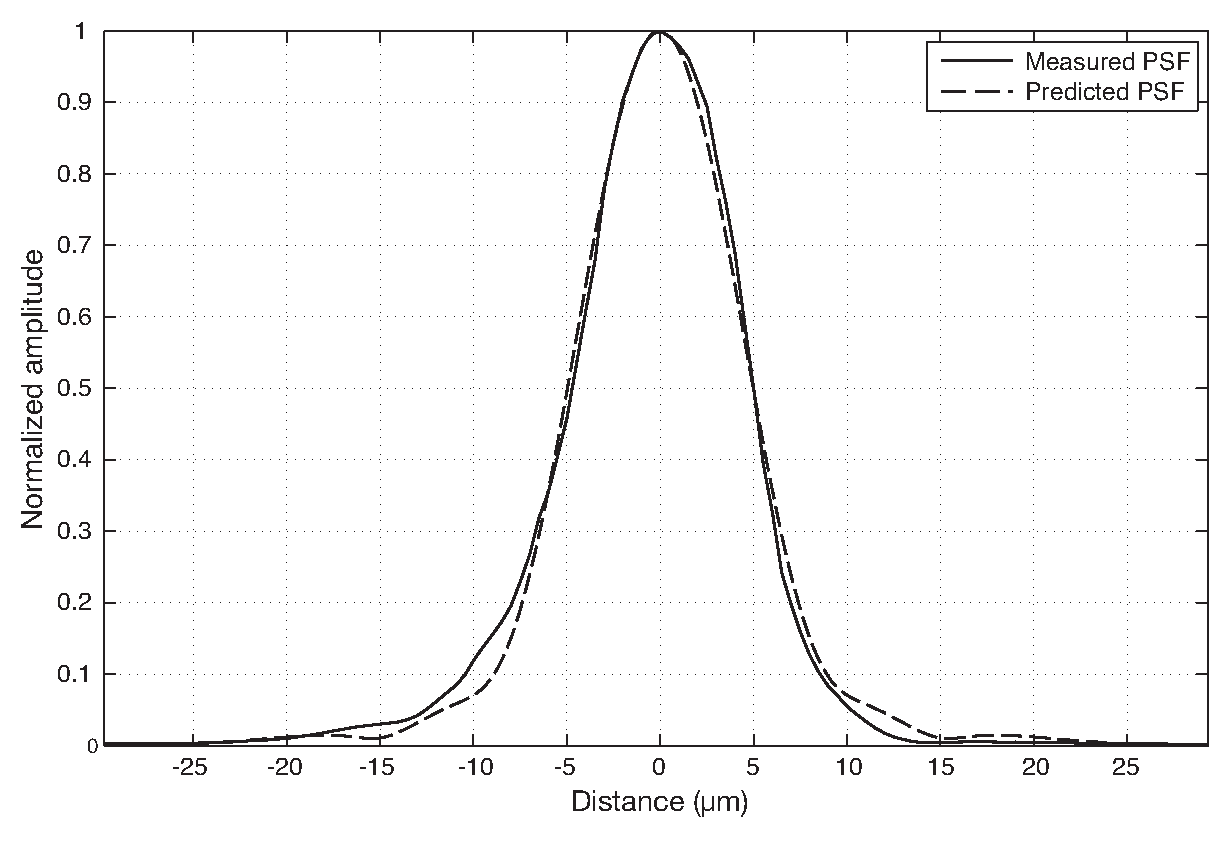
\includegraphics[width=0.8\textwidth]{Images/Results/psf-aom2.eps}
\caption[The measured axial point spread function.]{The measured axial point spread function of the FO-DOCM system. The measured PSF is shown as a solid line, and the predicted PSF as a dashed line.\label{fig:psf_comparison}}
\end{figure}

\subsection{Measurement of transverse resolution}

The fiber DOCM system is not designed for en-face (transverse) scanning, so verifying the transverse resolution was significantly more difficult. To do this, two methods were used: an en-face scan of a standard 1951 USAF resolution test target, and a cross-sectional scan of the edge of a microscope coverslip.

\begin{figure}[h!]
\centering
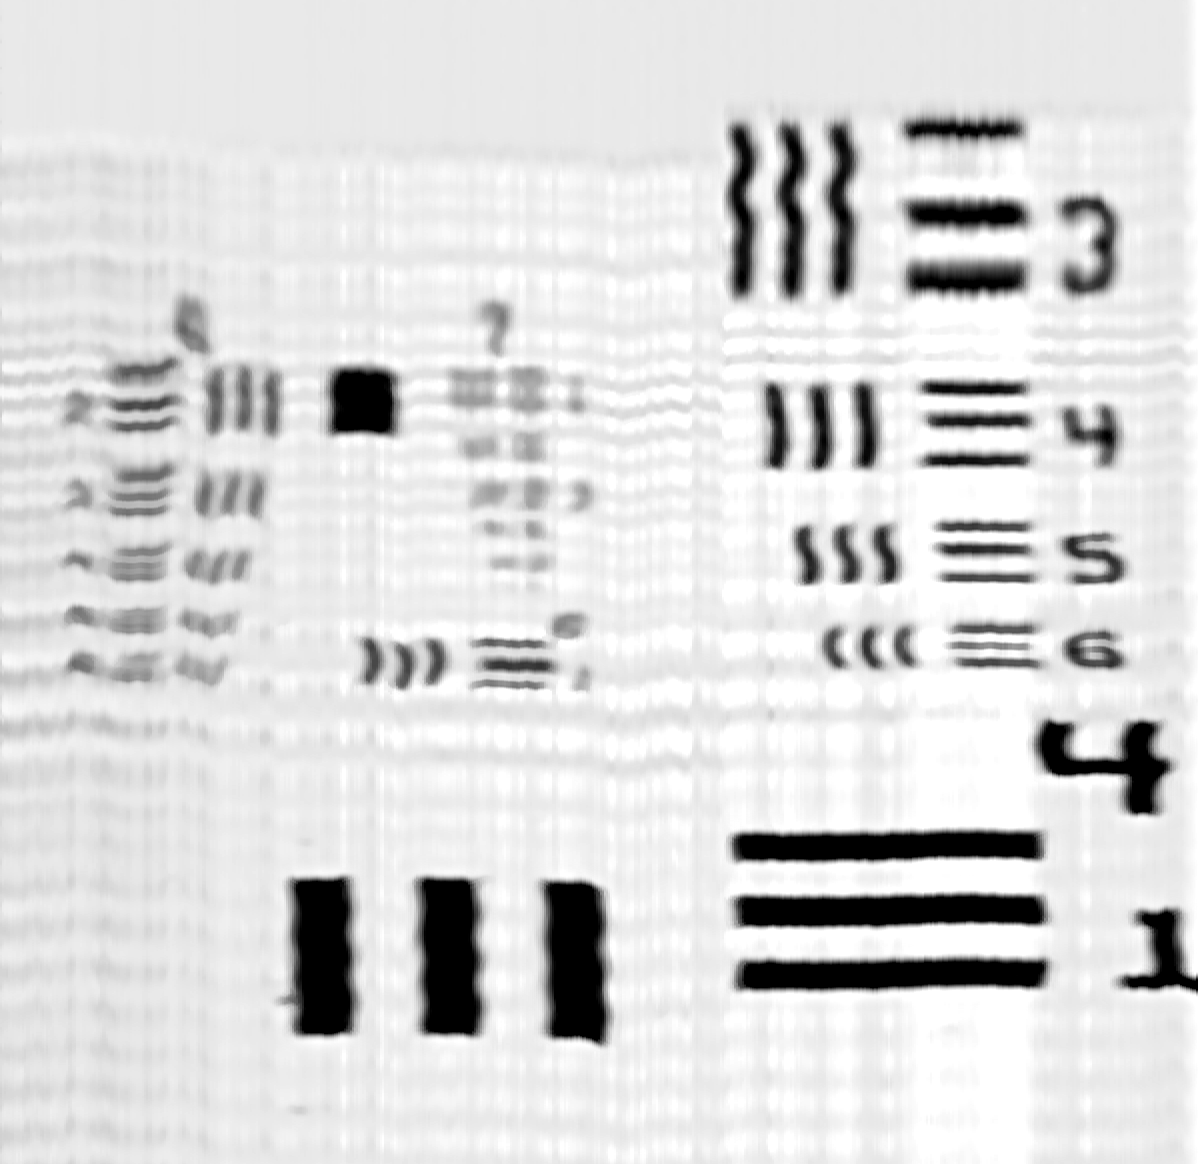
\includegraphics[width=0.5\textwidth]{Images/Results/en-face-usaf.png}
\caption[Result of en-face scan of USAF target.]{Result of en-face scan of 1951 USAF target. Note the distortion caused by the variable speed and low repeatability on the transverse stepper motor stage. Despite the distortion, all of the elements of Group 6 are distinguishable, indicating a transverse resolution of approximately 8.8 microns.\label{fig:usaf_oct}}
\end{figure}

Shown in Figure~\ref{fig:usaf_oct}, the USAF resolution test target was imaged by holding the fiber DOCM system at a constant z-axis depth, and recording the photodiode signal while moving the y-axis continuously. Then, the x-axis was incremented by 1 micron, and the process repeated. Because the transverse stage was not chosen for suitability for this type of scanning, severe distortion is visible in the result due to the acceleration and deceleration of the stage during the y-axis scan. Point-by-point scanning was not possible due to thes slow speed of the transverse stage. Vertical re-alignment of each column was performed to correct for poor repeatability in the stage, and a median filter was applied to reduce noise. Despite the clear unsuitability of this method of scanning for imaging applications, the visibility of all elements of group 6 within the USAF resolution test target in this experiment indicates a transverse resolution of approximately 8.8 microns.

\begin{figure}[h!]
\centering
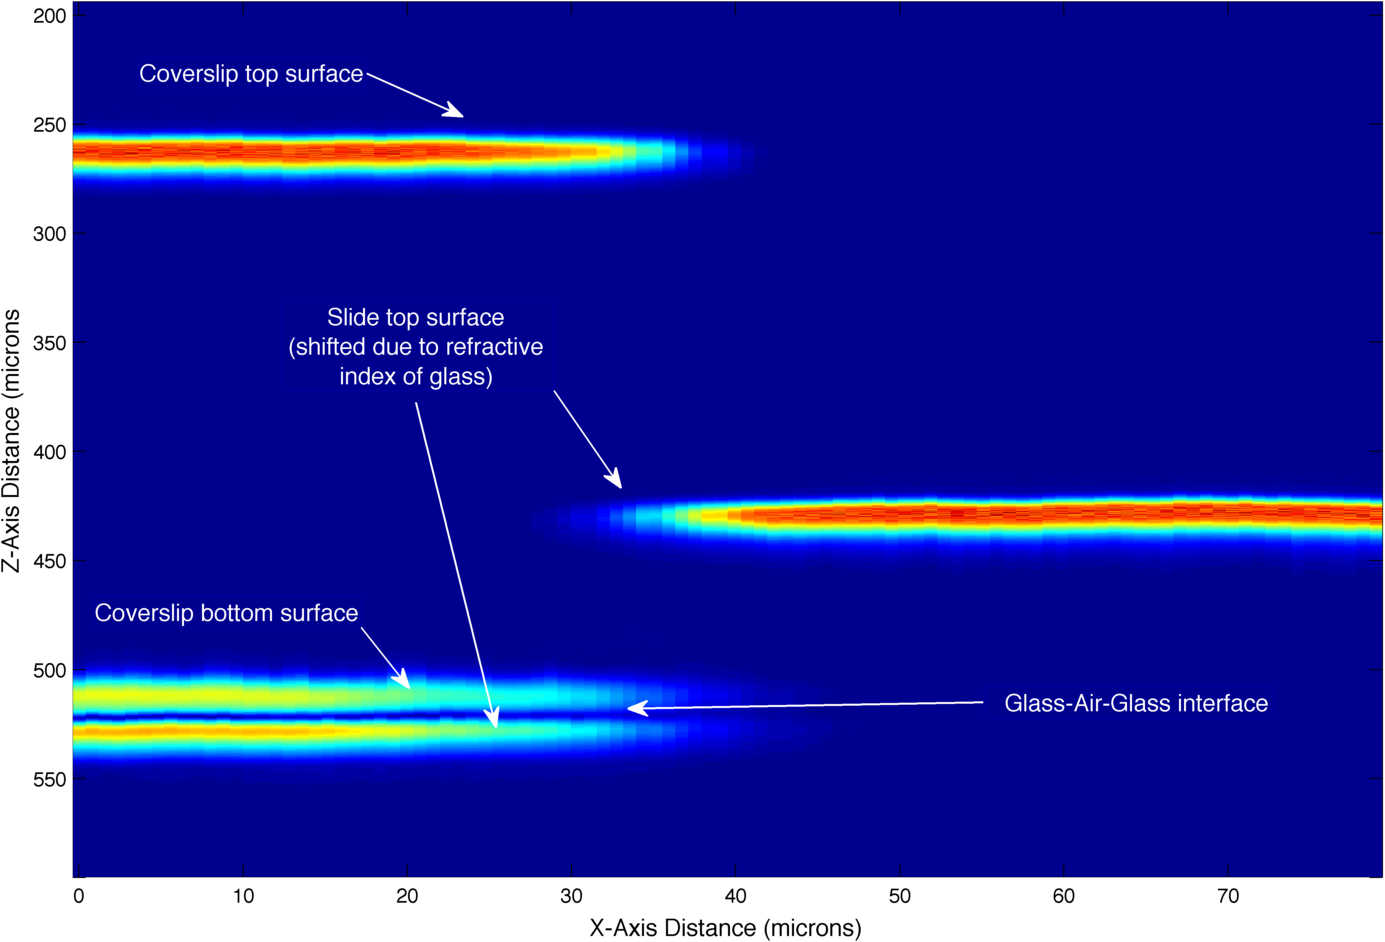
\includegraphics[height=230pt]{Images/Results/coverslip_ann.png}
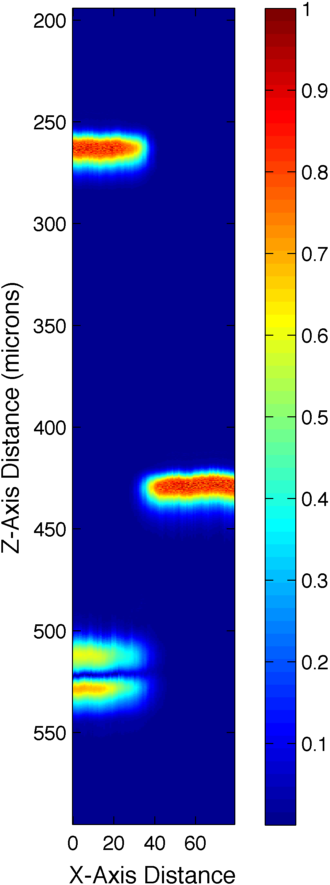
\includegraphics[height=230pt]{Images/Results/coverslip_equal.png}
\caption[Result of scan of the edge of a a glass coverslip.]{Result of scan of the edge of a a glass coverslip, with major features labeled. On the right is the same image, with 1:1 scaling between the x and z axes.\label{fig:coverslip1}}
\end{figure}

To obtain a less distorted measure of the transverse resolution of the fiber DOCM system, a second experiment was performed. In this experiment, shown in Figure~\ref{fig:coverslip1}, the edge of a microscope coverslip, resting on a microscope slide, was imaged in the x-z plane. The transition between the coverslip and air is the transverse step function of the system. Theoretically, this step function could be differentiated to obtain the transverse point spread function. However, differentiation increases noise, which renders this PSF unsuitable. Instead, the integral of a Gaussian function, an error function, can be fitted to the step function, as shown in Figure~\ref{fig:coverslip2}. The best fit parameters correspond to a transverse FWHM resolution of $9 \pm 0.7$ microns, which corroborates the USAF target image.

\begin{figure}[h!]
\centering
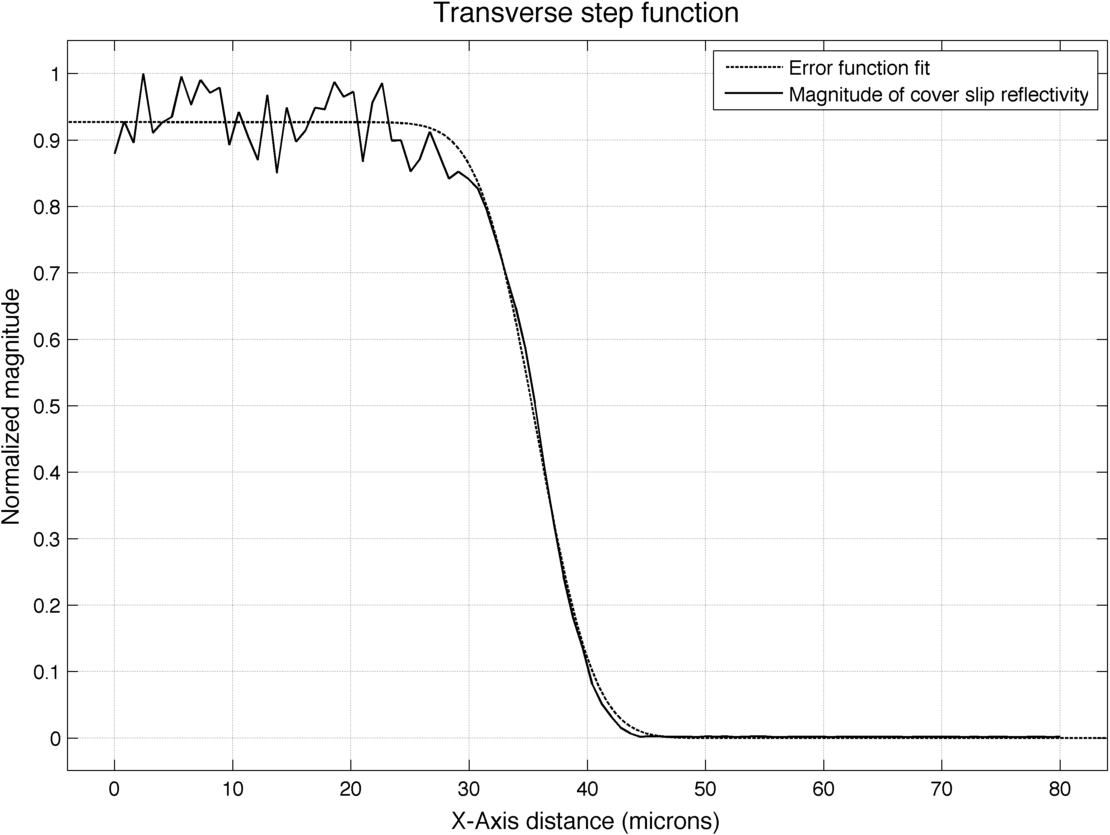
\includegraphics[width=0.8\textwidth]{Images/Results/line_step.png}
\caption[Transverse step function measured along the glass coverslip.]{Transverse step function measured along the glass coverslip. This corresponds to a single horizontal line in Figure~\ref{fig:coverslip1}. The best fit error function (the integral of a Gaussian) corresponds to a FWHM resolution of $9 \pm 0.7$ microns, corroborating the USAF target experiment.\label{fig:coverslip2}}
\end{figure}

\subsection{Limits of motion measurements}

To measure the noise floor of motion measurements, the sample path was focused onto a fixed aluminum front-surface mirror. 
% The spectral density noise floor of this signal is shown in Figure~\ref{fig:noise_floor1}. Above approximately 2 KHz, the effective noise floor for motion resolution with a sample reflectivity of 1 is shown to be 2 pm/Hz$^{0.5}$.
To more accurately simulate the reflectivity of tissues, a $10^{-2}$ attenuator was inserted into the optical path, attenuating the sample signal by $10^{-4}$. The acquired photodiode signal was analyzed according to the process outlined in Section~\ref{sec:motion_analysis_2}. The spectral density of this signal is shown in Figure~\ref{fig:noise_floor2}.
%After adjusting the reference path reflectivity to match, there was little difference in the effective motion noise floor.
Above 3 KHz, a noise floor of approximately 1 pm/Hz$^{0.5}$ was measured.

The strong impulsive frequencies present above 10 KHz are caused by electromagnetic interference in the analog-to-digital converter, originating from the computer hosting it, and not any inherent issues with the FO-DOCM system. Below 4 KHz, the frequencies could be the result of mechanical vibrations. An effort to further explain the presence of these frequencies is made in Section~\ref{sec:known_issues}. Because of this interference, stimulus frequencies of 1 KHz, 4 KHz, and 16 KHz were used in further testing. % justify this?

% \begin{figure}[h!]
% \centering
% 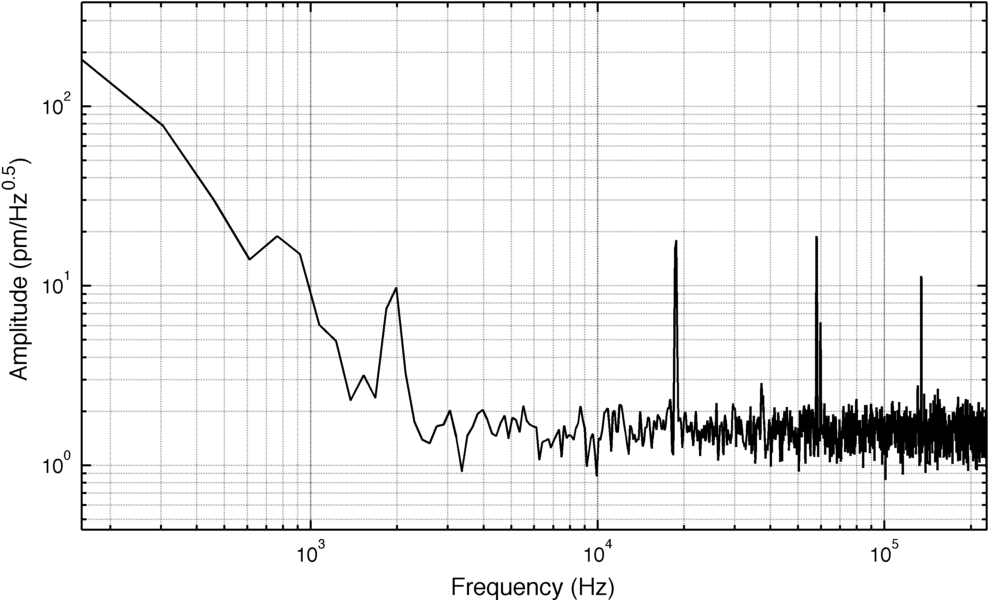
\includegraphics[width=0.75\textwidth]{Images/Results/noise_floor_r1_sm.png}
% \caption[Noise floor of motion measurement with sample reflectivity of approximately $1$.]{Noise floor of motion measurement with sample reflectivity of approximately $1$. The noise floor above 2 KHz is approximately 2 pm/Hz$^{0.5}$. The impulsive peaks are the result of electromagnetic interference in the analog-to-digital converter. \label{ref:noise_floor1}}
% \end{figure}

\begin{figure}[h!]
\centering
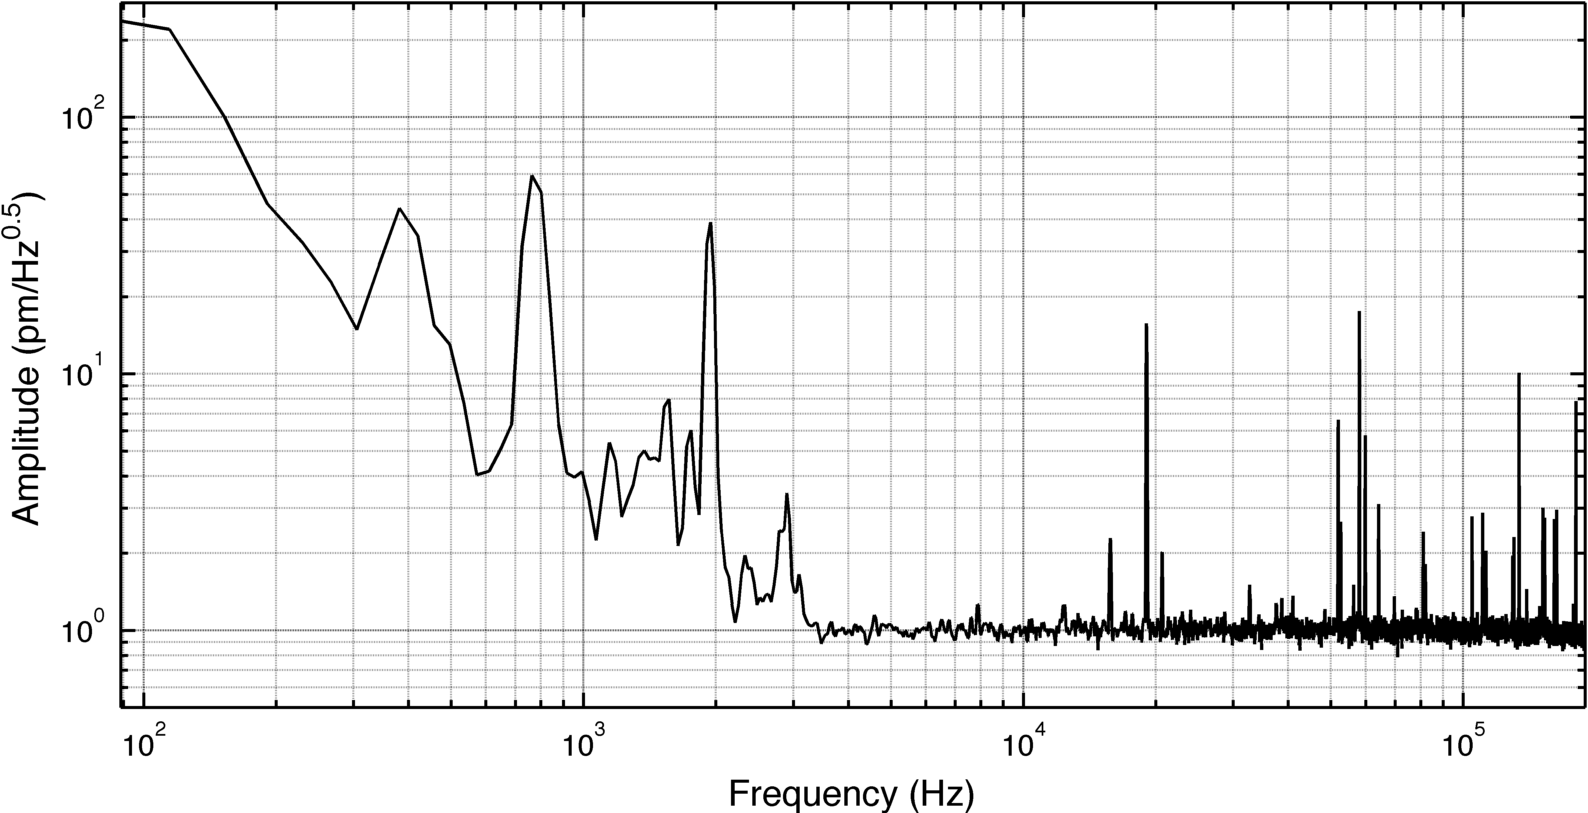
\includegraphics[width=0.95\textwidth]{Images/Results/noise_floor_2_big.png}
\caption[Noise floor of motion measurement with sample reflectivity of approximately $10^{-4}$.]{Noise floor of motion measurement with sample reflectivity of approximately $10^{-4}$. The noise floor above 3 KHz is approximately 1 pm/Hz$^{0.5}$. The impulsive peaks are the result of electromagnetic interference between the ADC and the computer hosting it. \label{fig:noise_floor2}}
\end{figure}

To verify the linearity of the motion measurements, a piezo-electric actuator was imaged while excited at a range of voltages. As the response of the piezo-electric actuator is very linear, the motion amplitude should increase linearly with increasing stimulus. \cite{klaassen} The response of the FO-DOCM system was shown to be linear over motion amplitudes ranging from approximately 200 picometers to 80 nanometers. Measured amplitude values and the best zero-intercept linear regression for each are shown in Figure~\ref{fig:motion_linearity}. Maximum deviation from the linear regression was $<2\%$ above 10 nm of motion, and for the 4 KHz stimulus, was $<5\%$ over the entire range. The root mean square error from the linear regression, for all frequencies, was 0.06 nm for amplitudes less than 10 nm, and 0.1nm over the entire amplitude range.

\begin{figure}[h!]
\centering
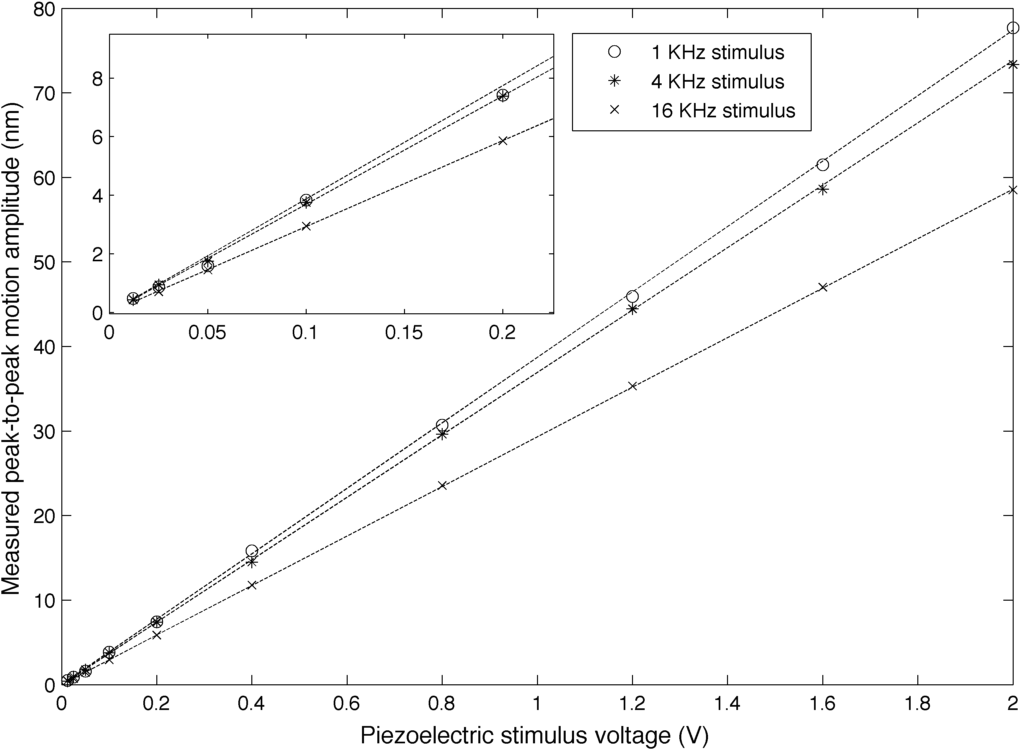
\includegraphics[width=0.75\textwidth]{Images/Results/motion_linearity.png}
\caption{Linearity of motion amplitude measurements.\label{fig:motion_linearity}}
\end{figure}

\subsection{Resolution of motion differentiation}

Another important system characteristic for analysis of cochlear motion is referred to as ``motion differentiation resolution'' -- the ability of the system to resolve the difference in vibrational amplitude between closely spaced objects. For this experiment, a glass coverslip was held just above a small ball-bearing glued to a piezo electric crystal. A sequence of reflectance and motion magnitude images were made, while the distance between the ball bearing and the coverslip was gradually reduced. The motion at the center of the ball bearing signal and at the center of the coverslip signal is plotted in Figure~\ref{fig:diff}. Motion measurements were taken as the median, over a $3 \times 1$ micron area, of the the amplitude of the best cosine fit to the analyzed distance signal. It should be noted that the reflected amplitude from the coverslip was approximately 10\% that of the reflected amplitude from the ball bearing.

\begin{figure}[h!]
\centering
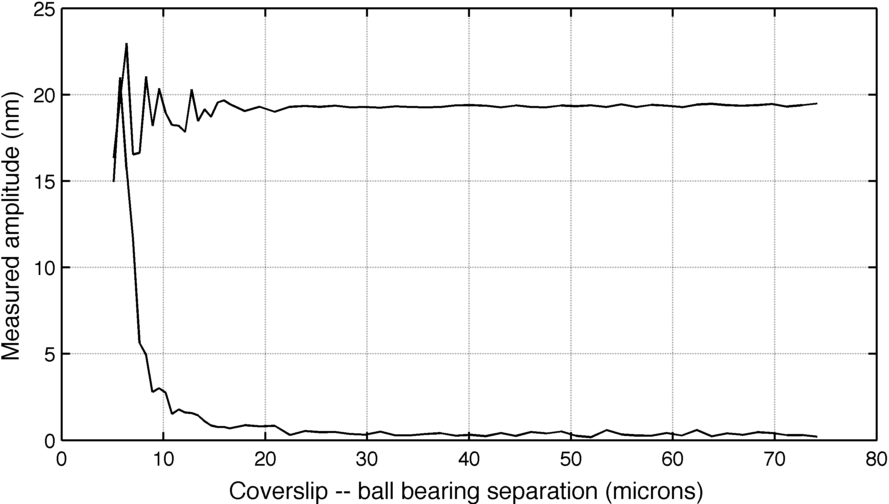
\includegraphics[width=0.85\textwidth]{Images/Results/differentiation.png}
\caption[Motion differentiation of adjacent stationary and vibrating interfaces.]{Motion differentiation of adjacent stationary and vibrating interfaces (coverslip and ball-bearing, respectively), measured with the FO-DOCM system.\label{fig:diff}}
\end{figure}

The motion amplitude between adjacent surfaces is shown to be differentiable for distances greater than approximately $7$ microns. This is expectedly close to the transverse FWHM resolution of approximately $9$ microns.

\section{Demonstrative images and motion measurements}

[This section has not yet been completed.]

\begin{figure}[h!]
\centering

\includegraphics[width=1.0\textwidth]{Images/missing.png}
\caption[An annotated guinea pig cochlea, imaged with the FO-DOCM system.]{An annotated guinea pig cochlea, imaged with the FO-DOCM system. As the motion induced by the piezo-electric actuator has an amplitude on the order of 10 nm, it does not result in visible artifacts in this image. \label{fig:cochlea_image}}
\end{figure}

% Table indicating motion measurements from this fixed cochlea.
\begin{table}[h!]
\centering
\begin{tabular}{l | c c}
Location & Amplitude (nm) & Phase (rad) \\ \hline
OHC & ? & ? \\
BMa & ? & ? \\
BMp & ? & ? \\
TM & ? & ? \\
RM & ? & ? \\
Bone & ? & ? \\
\end{tabular}
\caption[Motion analysis of fixed cochlea.]{Motion analysis of fixed cochlea. The cochlea was stimulated with a piezo-electric transducer at 4.0 KHz. Results were averaged over a $9 \times 9$ micron area (corresponding to $3 \times 3$ pixels in Figure~\ref{fig:cochlea_image}). \label{tab:cochlea_vib}}
\end{table}

A guinea pig cochlea was prepared by fixing in Glutaraldehyde. The cochlea was adhered with dental cement to a petri dish, which was excited by a piezo-electric transducer, with a stimulus frequency of 2.0 KHz. The cochlea was imaged by the FO-DOCM system over an $501 \times 501$ micron area, with pixel size of $3 \times 3$ microns. The log reflectivity over this area is shown in Figure~\ref{fig:cochlea_image}. The amplitude and phase of vibration at several labeled sites is shown in Table~\ref{tab:cochlea_vib}. These motion parameters were averaged over a $9 \times 9$ micron area.

\section{Known issues}
\label{sec:known_issues}

% \paragraph{Scanning speed}

% Currently, the FO-DOCM system does not offer significant improvements in the speed of image and motion acquisition compared to the Hong system, its predecessor in the Micromechanics Group. \cite{hong}

\paragraph{Stage repeatability}

The transverse stepper motor stage has quite poor repeatability, as became apparent during the en-face experiment to measure transverse resolution limits. While this is not a problem for unidirectional x-z or y-z scans, it prevents the use of the apparatus for en-face scanning or for accurate three dimensional scanning.

The z-axis piezo motor stage was also shown to have less reliable repeatability than originally intended. While the manufacturer's quoted bi-directional repeatability specification was 0.2 microns, in practice a repeatability of 2 microns is achieved. The cause of this order of magnitude disparity between quoted specifications and apparent performance is currently unknown. While this repeatability is sufficiently below the resolution limit of the FO-DOCM device to allow it to be functional for scanning, improving the repeatability of this stage would improve the resulting image quality.

\paragraph{Transverse resolution}

The transverse resolution measured of the FO-DOCM system was significantly worse than the predicted value from Zemax, by approximately a factor of two. This performance degradation must be caused by a problem with the GRIN lens assembly used for focusing the optical sample path. As shown in Figure~\ref{fig:grin_assembly}, the GRIN lens has an 8 degree face angle to reduce back-reflections. If this face angle were axially misaligned, it could result in optical aberrations that would degrade performance. Furthermore, any uncleanliness on interior surfaces of the assembly might degrade performance and would be impossible to clean after the optical adhesive has set. It is therefore theorized that some combination of the above issues is responsible for the degraded transverse resolution performance, and that the issue would be resolved by the construction of a new GRIN lens assembly.

\paragraph{Signal-to-noise ratio}

The noise floor of motion measurements shows significant interference at particular frequencies, though the overall noise floor is quite low. It is believed that much of the higher noise floor at these particular frequencies results from electromagnetic interference between the analog-to-digital conversion PCI card, and the computer that hosts it. To test this assumption, a signal was acquired from the analog-to-digital converter while the converter was connected only to a 50 ohm terminator. This power spectrum shows frequency peaks explaining the 16 KHz, 19 KHz, and higher peaks in Figure~\ref{fig:noise_floor2}. As the signal was acquired with the inputs immediately terminated, the source of this interference is most likely to be inside the computer itself, and would require a different analog-to-digital converter to eliminate. % Include graph? Test this again?

The lower peaks in noise, at 380 Hz, 760 Hz and 1950 Hz, are still of unknown origin. Mechanical vibration and noise becomes more likely at lower frequencies. To limit mechanical vibration, vibration damping washers could be employed on the fasteners in the alignment apparatus. The peaks could also be the result of sidebands or distortion in the RF synthesizer output. Further investigation and debugging is required if the FO-DOCM system is to become useful for measuring small amplitude motion at frequencies less than 3 KHz.

% Mechanical resonances?

\section{Conclusion}

The design and implementation a fiber optic doppler optical coherence microscopy (FO-DOCM) system for use in cochlear imaging was presented. The FO-DOCM system uses a fiber optic design to reduce system size and complexity and a novel alignment and micropositioning apparatus can increase the ease of use for the researcher performing the imaging. To enable precise motion measurements, a time domain approach is used, utilizing an acousto-optic modulator (AOM) based optical heterodyne system to generate a stationary interference carrier frequency.

This system is shown to be capable of measuring motion with magnitude on the order of $10$ picometers, competitive with or better performance than most published doppler optical coherence tomography systems. In addition to interferometrically measuring small amplitude motion, the FO-DOCM system is shown to be capable of imaging with a volumetric resolution of $10 \times 9 \times 9$ microns. Results of imaging cochlear tissue {\em in vitro} using the FO-DOCM system have been presented, showing its suitability for cochlear imaging. The FO-DOCM system will continue to be used and developed by the Micromechanics Group for use in cochlear research.
